% 图 7.1 —— 由 `checks/emit_hand.py` 自动拼出（probe 精测 + prims2 图元分解）
%%
% ⚠ 这是**稿子不是成品**：跑 `checks/checkhand.py 7.1` 看指标 + 看叠合图。
%%
%% ⚠ 待核：
%   · 本图 probe 报出阴影族 1 个 —— **本脚本不生成阴影**（要照原书手写）；prims2 的 strokes 里可能含阴影线，核对时留意别画重
%   · 可疑字形 3 项（空心圈 ⊙ 常被认成字母 o）—— 见文件末
%%
\documentclass[12pt]{standalone}
\usepackage{fontspec}
\setsansfont{Arial}
\newfontfamily\mfallback{DejaVu Sans}
\usepackage{tikz}
\begin{document}
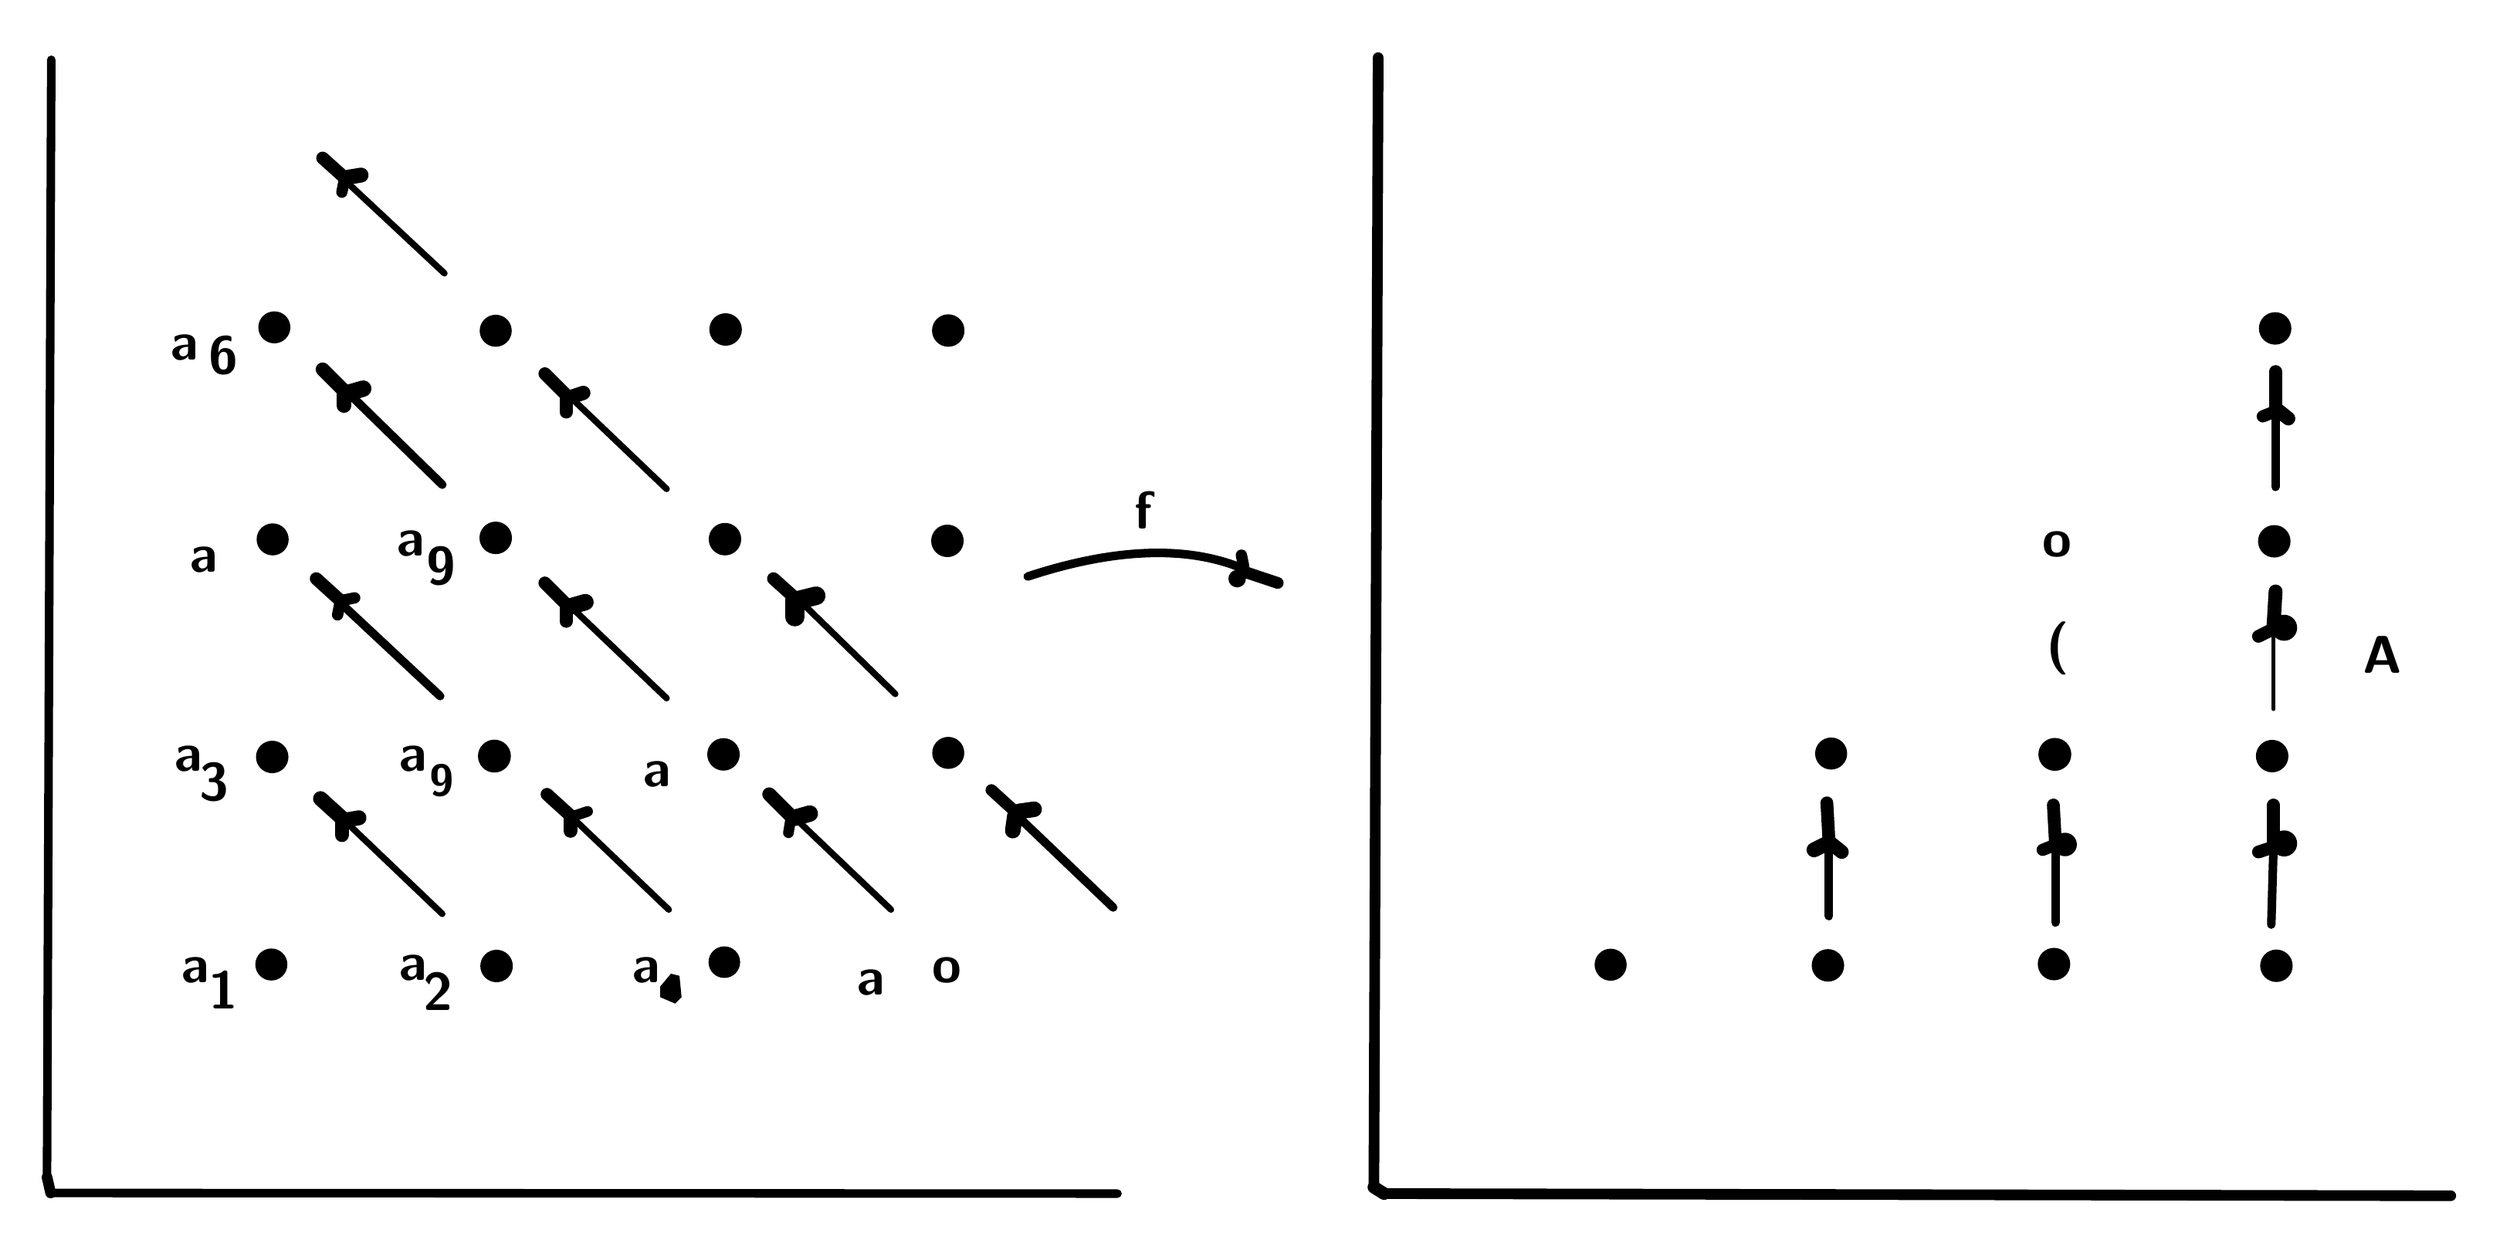
\begin{tikzpicture}[x=1pt, y=-1pt, line width=5.7pt, line cap=round, line join=round]

  %% ════ 填充区（prims2 的 fills）════
  \fill (304.0,446.0) -- (299.0,452.0) -- (299.0,457.0) -- (306.0,460.0) -- (309.0,457.0) -- (308.0,447.0) -- cycle;

  %% ════ 直线段（prims2 的 strokes）════
  \draw[line width=5.7pt] (1054.0,183.0) -- (1049.0,185.0);
  \draw[line width=6.7pt] (151.0,174.0) -- (151.0,180.0);
  \draw[line width=3.0pt] (302.0,219.0) -- (257.0,176.0);
  \draw[line width=6.0pt] (255.0,275.0) -- (255.0,281.0);
  \draw[line width=7.7pt] (369.0,371.0) -- (362.0,373.0);
  \draw[line width=4.0pt] (1053.0,423.0) -- (1054.0,388.0);
  \draw[line width=4.0pt] (1055.0,184.0) -- (1055.0,218.0);
  \draw[line width=3.0pt] (303.0,416.0) -- (258.0,373.0);
  \draw[line width=7.7pt] (153.0,174.0) -- (160.0,172.0);
  \draw[line width=4.0pt] (153.0,174.0) -- (197.0,217.0);
  \draw[line width=3.0pt] (362.0,373.0) -- (407.0,416.0);
  \draw[line width=3.0pt] (409.0,315.0) -- (364.0,271.0);
  \draw[line width=3.0pt] (152.0,375.0) -- (197.0,418.0);
  \draw[line width=6.5pt] (141.0,163.0) -- (151.0,173.0);
  \draw[line width=6.5pt] (350.0,362.0) -- (360.0,372.0);
  \draw[line width=6.5pt] (1055.0,267.0) -- (1054.0,284.0);
  \draw[line width=7.3pt] (474.0,369.0) -- (467.0,370.0);
  \draw[line width=5.0pt] (265.0,370.0) -- (259.0,372.0);
  \draw[line width=5.3pt] (149.0,273.0) -- (148.0,278.0);
  \draw[line width=3.0pt] (302.0,317.0) -- (257.0,274.0);
  \draw[line width=7.0pt] (845.0,385.0) -- (839.0,388.0);
  \draw[line width=6.0pt] (1047.0,389.0) -- (1053.0,387.0);
  \draw[line width=5.7pt] (1053.0,246.0) -- (1056.0,242.0);
  \draw[line width=8.7pt] (362.0,271.0) -- (362.0,279.0);
  \draw[line width=6.0pt] (1053.0,285.0) -- (1047.0,288.0);
  \draw[line width=4.0pt] (14.0,18.0) -- (12.0,541.3);
  \draw[line width=5.0pt] (12.0,541.3) -- (13.7,548.7);
  \draw[line width=4.0pt] (13.7,548.7) -- (513.0,549.0);
  \draw[line width=4.0pt] (952.0,422.0) -- (952.0,387.0);
  \draw[line width=4.0pt] (466.0,372.0) -- (511.0,415.0);
  \draw[line width=6.0pt] (151.0,73.0) -- (141.0,64.0);
  \draw[line width=5.0pt] (1137.0,550.0) -- (637.8,549.0);
  \draw[line width=5.9pt] (637.8,549.0) -- (633.0,546.0);
  \draw[line width=5.0pt] (633.0,546.0) -- (635.0,17.0);
  \draw[line width=6.5pt] (847.0,385.0) -- (852.0,389.0);
  \draw[line width=8.7pt] (364.0,271.0) -- (372.0,269.0);
  \draw[line width=5.3pt] (151.0,75.0) -- (150.0,80.0);
  \draw[line width=2.0pt] (1054.0,286.0) -- (1054.0,322.0);
  \draw[line width=6.5pt] (1061.0,186.0) -- (1056.0,182.0);
  \draw[line width=7.0pt] (158.0,373.0) -- (152.0,374.0);
  \draw[line width=6.7pt] (150.0,381.0) -- (150.0,375.0);
  \draw[line width=7.0pt] (153.0,73.0) -- (159.0,72.0);
  \draw[line width=7.3pt] (464.0,379.0) -- (465.0,372.0);
  \draw[line width=6.0pt] (245.0,165.0) -- (255.0,175.0);
  \draw[line width=5.7pt] (951.0,386.0) -- (946.0,388.0);
  \draw[line width=6.0pt] (149.0,271.0) -- (138.0,261.0);
  \draw[line width=6.0pt] (952.0,385.0) -- (951.0,367.0);
  \draw[line width=5.0pt] (360.0,374.0) -- (359.0,380.0);
  \draw[line width=4.0pt] (846.0,386.0) -- (846.0,419.0);
  \draw[line width=7.7pt] (257.0,274.0) -- (264.0,272.0);
  \draw[line width=5.3pt] (151.0,271.0) -- (156.0,270.0);
  \draw[line width=5.5pt] (465.0,370.0) -- (454.0,360.0);
  \draw[line width=6.0pt] (1055.0,164.0) -- (1055.0,181.0);
  \draw[line width=6.0pt] (362.0,270.0) -- (352.0,261.0);
  \draw[line width=6.0pt] (845.0,366.0) -- (846.0,384.0);
  \draw[line width=6.0pt] (257.0,372.0) -- (246.0,362.0);
  \draw[line width=5.5pt] (588.0,263.0) -- (573.0,258.0);
  \draw[line width=6.0pt] (1054.0,367.0) -- (1054.0,385.0);
  \draw[line width=6.7pt] (257.0,176.0) -- (263.0,174.0);
  \draw[line width=6.0pt] (255.0,177.0) -- (255.0,183.0);
  \draw[line width=6.0pt] (245.0,263.0) -- (255.0,273.0);
  \draw[line width=5.3pt] (571.0,250.0) -- (572.0,255.0);
  \draw[line width=3.0pt] (198.0,118.0) -- (152.0,75.0);
  \draw[line width=6.7pt] (257.0,379.0) -- (257.0,373.0);
  \draw[line width=7.0pt] (151.0,374.0) -- (140.0,364.0);
  \draw[line width=4.0pt] (150.0,273.0) -- (196.0,316.0);

  %% ════ 曲线（prims2 的 curves —— 三段式，坐标同为 (y,x)）════
  \draw[line width=4.0pt] (471.0,260.0) .. controls (501.8,249.8) and (539.7,243.2) .. (571.0,256.0);

  %% ════ 实心点 ════
  \fill (118.4,143.3) circle (7.5);
  \fill (329.6,144.3) circle (7.6);
  \fill (1054.8,143.8) circle (7.6);
  \fill (222.0,144.9) circle (7.5);
  \fill (433.8,144.8) circle (7.6);
  \fill (222.0,241.9) circle (7.6);
  \fill (117.6,242.6) circle (7.5);
  \fill (329.3,242.5) circle (7.6);
  \fill (433.4,243.3) circle (7.6);
  \fill (1054.4,243.5) circle (7.6);
  \fill (328.6,343.3) circle (7.6);
  \fill (433.8,342.6) circle (7.5);
  \fill (847.0,342.9) circle (7.5);
  \fill (951.7,343.3) circle (7.7);
  \fill (117.4,344.5) circle (7.6);
  \fill (221.4,344.1) circle (7.7);
  \fill (1053.4,344.1) circle (7.6);
  \fill (329.0,440.6) circle (7.4);
  \fill (117.0,441.7) circle (7.5);
  \fill (222.4,442.4) circle (7.6);
  \fill (743.8,441.8) circle (7.5);
  \fill (845.5,442.1) circle (7.6);
  \fill (951.3,441.5) circle (7.6);
  \fill (1055.4,442.3) circle (7.6);
  \fill (569.0,261.0) circle (4.1);
  \fill (1059.0,284.0) circle (6.1);
  \fill (1059.0,385.0) circle (6.1);
  \fill (956.5,385.5) circle (5.5);

  %% ════ 标签（probe 直接给的 \node 行）════
  %% ⚠ 全部补了 fill=white：文字在最上层，否则与曲线交叉干扰
     \node[anchor=center,inner sep=0pt,fill=white,font=\fontsize{47.3}{59.1}\selectfont] at (76.6,152.9) {\textsf{\textbf{\textit{a}}}};   % box(64,137,22,27)
     \node[anchor=center,inner sep=0pt,fill=white,font=\fontsize{23.7}{29.6}\selectfont] at (94.6,156.6) {\textsf{\textbf{6}}};   % box(88,148,12,16)
     \node[anchor=center,inner sep=0pt,fill=white,font=\fontsize{29.1}{36.4}\selectfont] at (526.0,229.0) {\textsf{\textbf{\textit{f}}}};   % box(520,217,11,23)
     \node[anchor=center,inner sep=0pt,fill=white,font=\fontsize{30.0}{37.6}\selectfont] at (182.5,244.5) {\textsf{\textbf{\textit{a}}}};   % box(174,235,15,16)
     \node[anchor=center,inner sep=0pt,fill=white,font=\fontsize{51.4}{64.2}\selectfont] at (85.7,252.1) {\textsf{\textbf{\textit{a}}}};   % box(71,236,26,27)
     \node[anchor=center,inner sep=0pt,fill=white,font=\fontsize{28.6}{35.8}\selectfont] at (952.7,244.9) {\textsf{\textbf{\textit{o}}}};   % box(944,236,16,15)
     \node[anchor=center,inner sep=0pt,fill=white,font=\fontsize{24.4}{30.5}\selectfont] at (196.4,255.1) {\textsf{\textbf{9}}};   % box(189,246,12,17)
     \node[anchor=center,inner sep=0pt,fill=white,font=\fontsize{60.1}{75.1}\selectfont] at (953.0,293.5) {\textsf{\textbf{(}}};   % box(944,264,16,57)
     \node[anchor=center,inner sep=0pt,fill=white,font=\fontsize{29.6}{37.0}\selectfont] at (1105.2,296.5) {\textsf{\textbf{\textit{A}}}};   % box(1093,285,19,22)
     \node[anchor=center,inner sep=0pt,fill=white,font=\fontsize{30.0}{37.6}\selectfont] at (78.5,345.5) {\textsf{\textbf{\textit{a}}}};   % box(70,336,15,16)
     \node[anchor=center,inner sep=0pt,fill=white,font=\fontsize{30.0}{37.6}\selectfont] at (183.5,345.5) {\textsf{\textbf{\textit{a}}}};   % box(175,336,15,16)
     \node[anchor=center,inner sep=0pt,fill=white,font=\fontsize{52.3}{65.4}\selectfont] at (297.7,352.6) {\textsf{\textbf{\textit{a}}}};   % box(283,336,26,28)
     \node[anchor=center,inner sep=0pt,fill=white,font=\fontsize{24.0}{30.0}\selectfont] at (90.4,356.1) {\textsf{\textbf{3}}};   % box(84,347,12,17)
     \node[anchor=center,inner sep=0pt,fill=white,font=\fontsize{22.7}{28.3}\selectfont] at (196.8,355.6) {\textsf{\textbf{9}}};   % box(190,347,11,16)
     \node[anchor=center,inner sep=0pt,fill=white,font=\fontsize{30.0}{37.6}\selectfont] at (183.5,443.5) {\textsf{\textbf{\textit{a}}}};   % box(175,434,15,16)
     \node[anchor=center,inner sep=0pt,fill=white,font=\fontsize{51.4}{64.2}\selectfont] at (397.7,450.1) {\textsf{\textbf{\textit{a}}}};   % box(383,434,26,27)
     \node[anchor=center,inner sep=0pt,fill=white,font=\fontsize{30.0}{37.6}\selectfont] at (81.5,444.5) {\textsf{\textbf{\textit{a}}}};   % box(73,435,15,16)
     \node[anchor=center,inner sep=0pt,fill=white,font=\fontsize{30.0}{37.6}\selectfont] at (292.5,444.5) {\textsf{\textbf{\textit{a}}}};   % box(284,435,15,16)
     \node[anchor=center,inner sep=0pt,fill=white,font=\fontsize{28.6}{35.8}\selectfont] at (433.2,444.4) {\textsf{\textbf{\textit{o}}}};   % box(425,435,15,16)
     \node[anchor=center,inner sep=0pt,fill=white,font=\fontsize{23.0}{28.7}\selectfont] at (94.7,453.9) {\textsf{\textbf{1}}};   % box(88,446,8,15)
     \node[anchor=center,inner sep=0pt,fill=white,font=\fontsize{22.9}{28.7}\selectfont] at (195.1,454.4) {\textsf{\textbf{2}}};   % box(189,446,11,16)

  % 钉死画布：否则超出的图元/控制点会把页面撑大，1:1 回比就失准
  \pgfresetboundingbox
  \path[use as bounding box] (0,0) rectangle (1150,562);
\end{tikzpicture}
\end{document}

% ⚠ 待核清单（probe 拿不准，人眼过一遍）：
%   · 可疑字形：\node[anchor=center,inner sep=0pt,font=\fontsize{28.6}{35.8}\selectfont] at (952.7,244.9) {\textsf{\textbf{\te
%   · 可疑字形：\node[anchor=center,inner sep=0pt,font=\fontsize{28.6}{35.8}\selectfont] at (433.2,444.4) {\textsf{\textbf{\te
%   · 未识别/跳过：⑤ 跳过/未识别的字形
